\newpage
\section{Evidencia de trabajo de estudiantes durante el curso}

\subsection{Resultado de aprendizaje \#: 3a}
\label{sec:ra3a}
Actividad: Proyecto (parte 2) – Diseño e implementación
Descripción:
Ha sido contratado por la empresa YOOSHI S.A. para generar un estudio de tecnologías a ser incorporadas en ECUADOR. La empresa YOOSHI S.A. se encarga de proveer servicios de vanguardia a sus clientes, por lo que, antes de realizar las implementaciones realiza un estudio a fines de conocer los beneficios y privilegios a sus clientes como a la empresa. 

Se han contratado diferentes firmas (sub-contratante) para que ayuden ha realizar los estudios.

Para llevar a cargo esta segunda etapa, se necesita primero comprobar si ha existido algún cambio en la administración de las empresas, siendo estos, cambio en los grupos de trabajo y gerente de la empresa. En los respaldos de la empresa se tiene la siguiente estructura:  
\begin{itemize}
    \item Seguridad y privacidad en SDN: Explora enfoques innovadores para mejorar los aspectos de seguridad y privacidad de SDN. Esto podría implicar el diseño e implementación de protocolos de comunicación seguros, sistemas de detección de intrusiones o técnicas de cifrado específicamente adaptadas para entornos de SDN. - GRProyecto4
    \item Virtualización de funciones de red (NFV) en SDN: Explora enfoques innovadores para asignar y gestionar de manera dinámica las funciones de red virtuales (VNF) en una arquitectura de SDN, teniendo en cuenta factores como el balanceo de carga, el encadenamiento de servicios y la tolerancia a fallos. - GRProyecto2
    \item Ingeniería de tráfico inteligente en SDN: Investiga y desarrolla algoritmos y técnicas inteligentes para optimizar la ingeniería de tráfico en SDN. Esto podría implicar enfoques novedosos para el balanceo de carga de tráfico, la gestión de congestión y la provisión de calidad de servicio (QoS) en redes SDN para mejorar el rendimiento de la red y la experiencia del usuario. - GRProyecto1
    \item Integración de IoT con SDN: Explora la integración de dispositivos de Internet de las cosas (IoT) con SDN para permitir una gestión y control eficientes de las redes IoT. Investiga enfoques innovadores para manejar la implementación a gran escala, la movilidad y las limitaciones de recursos de los dispositivos IoT en entornos de SDN, teniendo en cuenta factores como la eficiencia energética, la escalabilidad y la confiabilidad. - GRProyecto3
\end{itemize}

Instrucciones:

Cada empresa sub-contratante a indicado de querer trabajar con un tema especifico que han hecho llegar a la empresa YOOSHI S.A. en días anteriores, para lo cuál se indican los siguientes requerimientos:

Utilizando el reporte de la primera sección (se puede utilizar el trabajo anterior, siempre y cuando se realicen los cambios sugeridos en la revisión) se debe:
\begin{itemize}
    \item Hacer un diseño esquemático de cómo implementarían la tecnología en la ciudad/zona/región que hayan estudiado en su primer reporte (Pueden utilizar lucidchart para realizar los diagramas - figuras e ilustraciones deben ser realizadas por cada empresa). Además, se deben utilizar en el diseño varios agentes de monitoreo, balanceo, administración, etc. que beneficien la implementación, y qué tipo de servicios en la nube van hacer provistos a los clientes (modelo SaaS, PaaS o IaaS).
    \begin{itemize}
        \item Este diseño contempla qué tipos de servidores, equipos, y sistemas operativos tendrá la estructura ha ser implementada en la ciudad/zona/región.
        \item Se debe tener un balance de los gastos que conllevan realizar la implementación. (Equipos, redes y mano de obra, mantenimiento, licencias, etc.) - Se verificará que los equipos sean actuales. 
        \item Dependiendo del modelo de diseño y de los agentes empleados, se debe dar la justificación de porque el uso de cada uno.
    \end{itemize}
    \item Se debe simular las redes de conectividad y la tecnología escogida, mediante cualquier escenario que la empresa decida, con la finalidad de convencer a YOOSHI S.A. de invertir en la solución. El entregable de la simulación debe ser un video donde se explique la solución, los beneficios y las tecnologías a utilizar. (Duración: 20min max.). - Solo la solución (Nada de teoría) - No se permite utilizar mininet
    \item El informe debe ser entregado en formato paper IEEE en latex - Se debe proveer a la empresa el informe final compartiendo el enlace del archivo latex al gerente de la empresa YOOSHI S.A. - Los grupos que no presenten el informe de Latex no pasarán a la presentación (i.e. Cero de calificación)
    \item El Informe debe ser mínimo seis (6) y máximo ocho (8) paginas
    \item El formato del articulo debe ser:
    \begin{itemize}
        \item TITULO (En inglés) Este debe estar acorde a la tecnología y al lugar especifico donde se realiza en estudio, puede ser una ciudad, una zona, una región, etc., pero, de Ecuador. 
        \item AUTORES
        \item ABSTRACT (En inglés), entre 100 - 150 palabras.
        \item INTRODUCCIÓN
        \item ESTADO DEL ARTE
        \item METODOLOGÍA - Diagramas o arquitectura computacional de cómo se implementa su solución.
        \item ANALISIS DE RESULTADOS - Escenarios de su solución describiendo métricas de análisis, e.g. tiempos de ejecución, memoria, disco, procesamiento, etc.
        \item DISCUSIÓN/CONCLUSIÓN - Se presenta la discusión de toda la solución y los escenarios, i.e., ventajas y desventajas que trae su modelo, la discusión se escribe como un ensayo argumentativo.
        \item BIBLIOGRAFIA 
    \end{itemize}

    \item Se deben crear Apéndices con la bitácora del proyecto y cualquier código que sea de utilidad para el entendimiento de la solución - Los apéndices no cuentan cómo extensión del documento original.


\end{itemize}

Finalizando, la elección del proyecto a implementarse en Ecuador se dará con una presentación a todos los participantes el día 25-08-2023 en horario de 11:00 - 12:30 am, donde cada empresa tendrá 10 minutos por reloj para convencer al jurado de la empresa. El jurado esta compuesto por miembros externos que tienen conocimiento del tema. Pueden revisar evaluaciones anteriores en:
\url{https://www.youtube.com/watch?v=tNPPbxmejpk}

La empresa YOOSHI S.A. para el correcto desarrollo del estudio provee a sus contratantes con la información que ellos puedan requerir, e.g., un articulo ó un capitulo de un libro. Estos dependiendo de los recursos y disponibilidad de la empresa YOOSHI S.A.

Para mayor información se pueden comunicar con el Gerente de Tecnología al correo wavelasq@espol.edu.ec  con el asunto SN\_PROYECTO.
La empresa YOOSHI S.A. les desea el mayor de los éxitos en esta ardua tarea. 

\subsubsection{Evidencia RA3a}
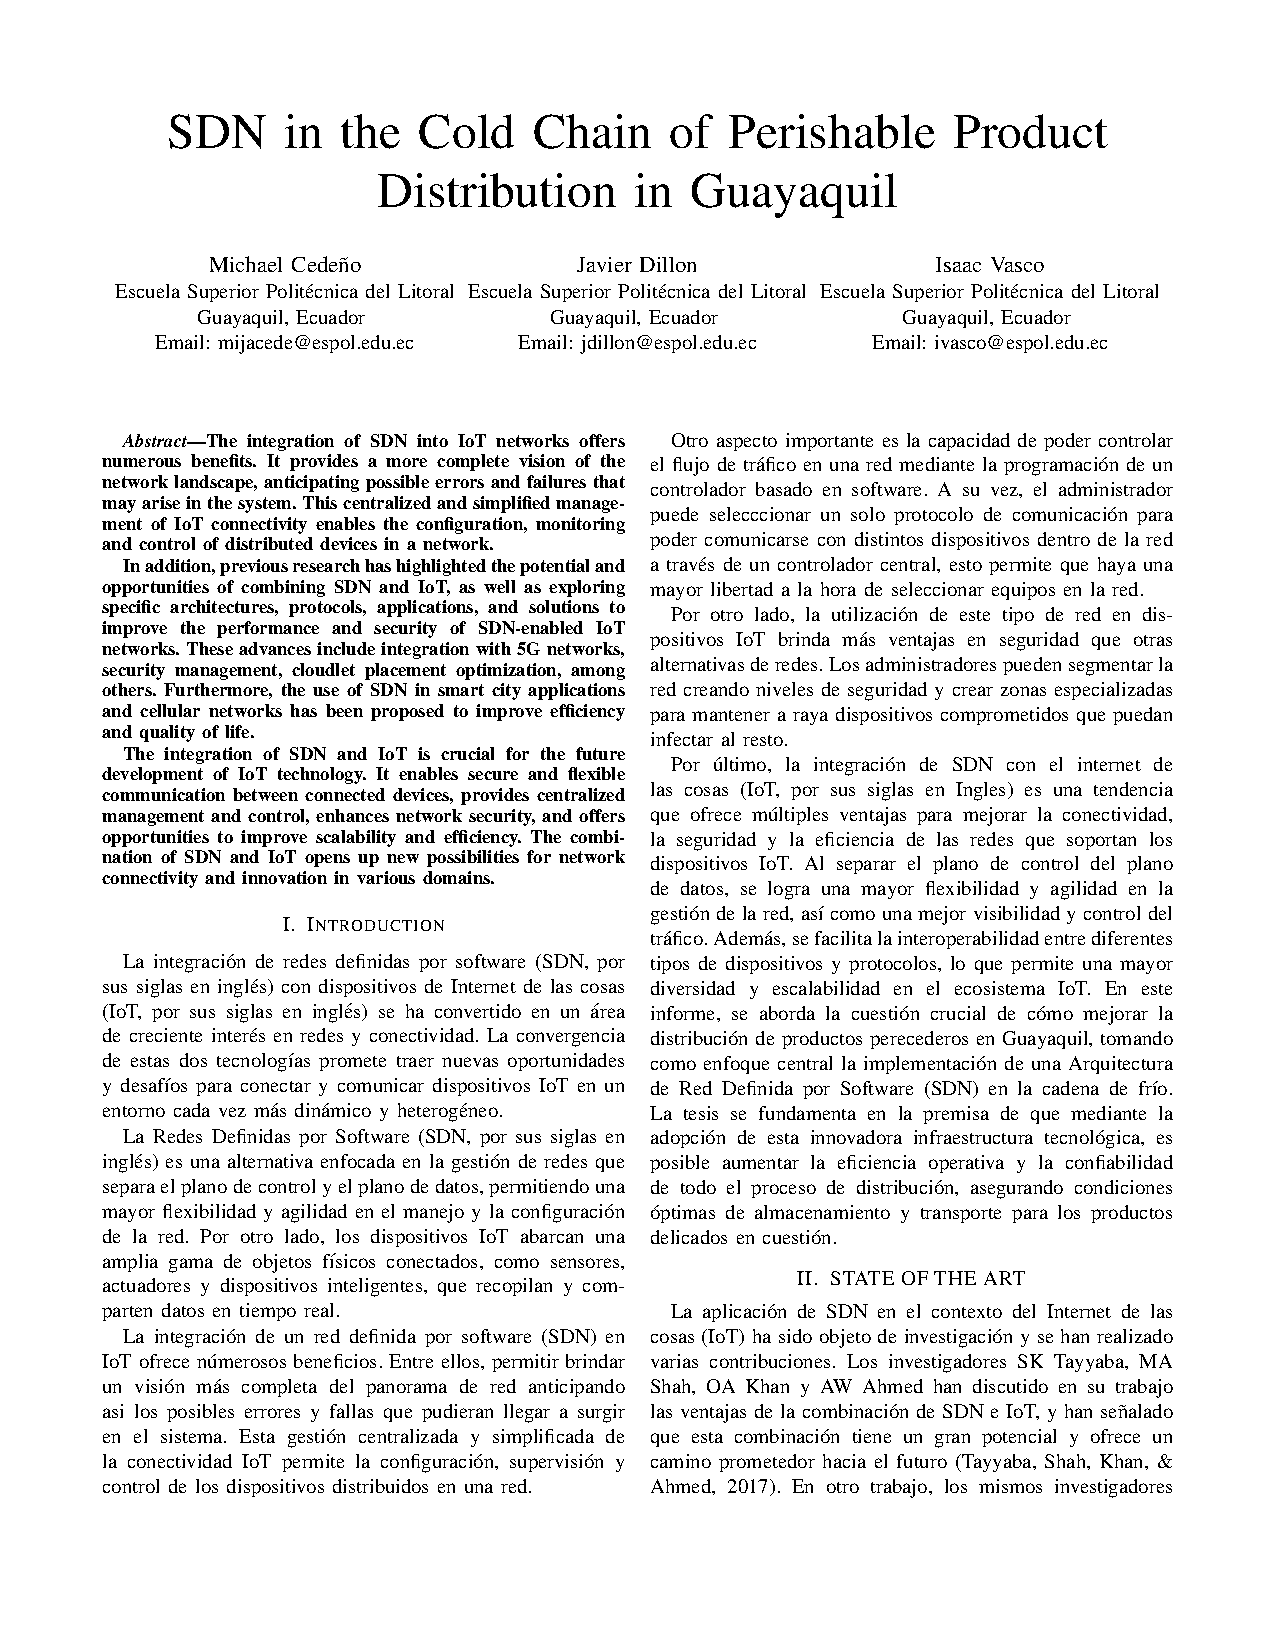
\includepdf[pages=-]{recursos/ra3/SDN_in_the_Cold_Chain.pdf}

\subsubsection{Retroalimentación RA3a}
\begin{figure}[!htbp]
    \centering
    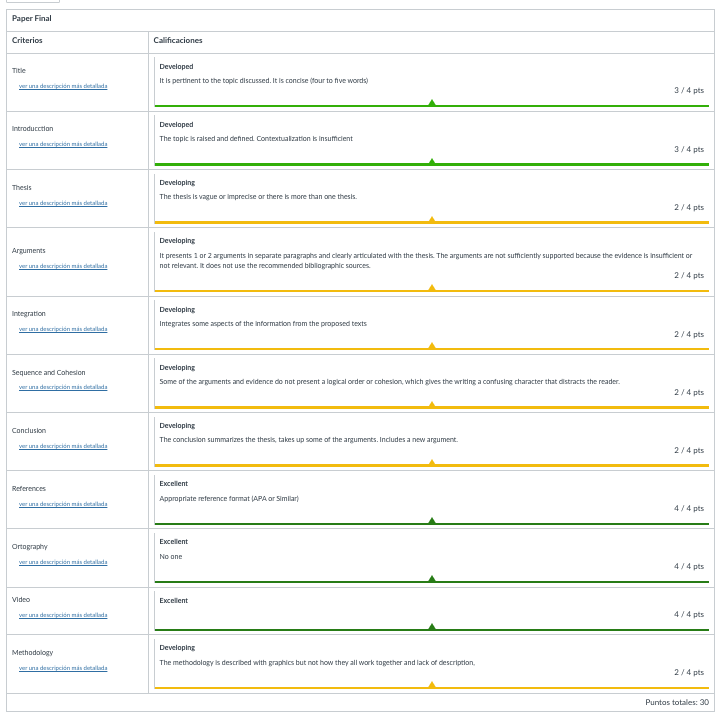
\includegraphics[width=\textwidth]{recursos/ra3/paper.png}
\end{figure}

\begin{figure}[!htbp]
    \centering
    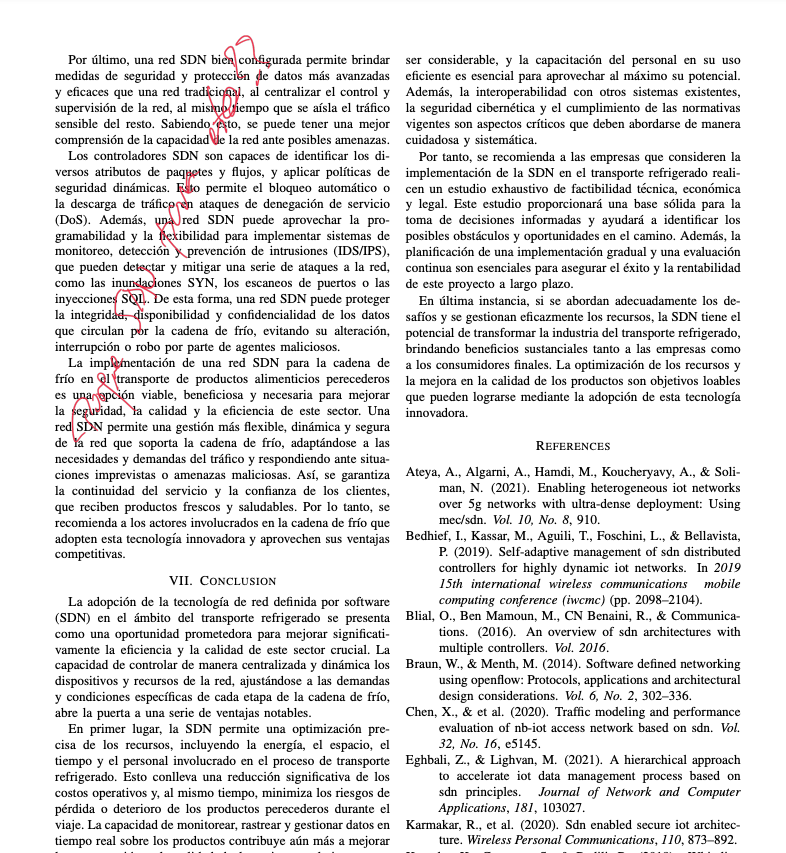
\includegraphics[width=\textwidth]{recursos/ra3/sto3a.png}
\end{figure}

%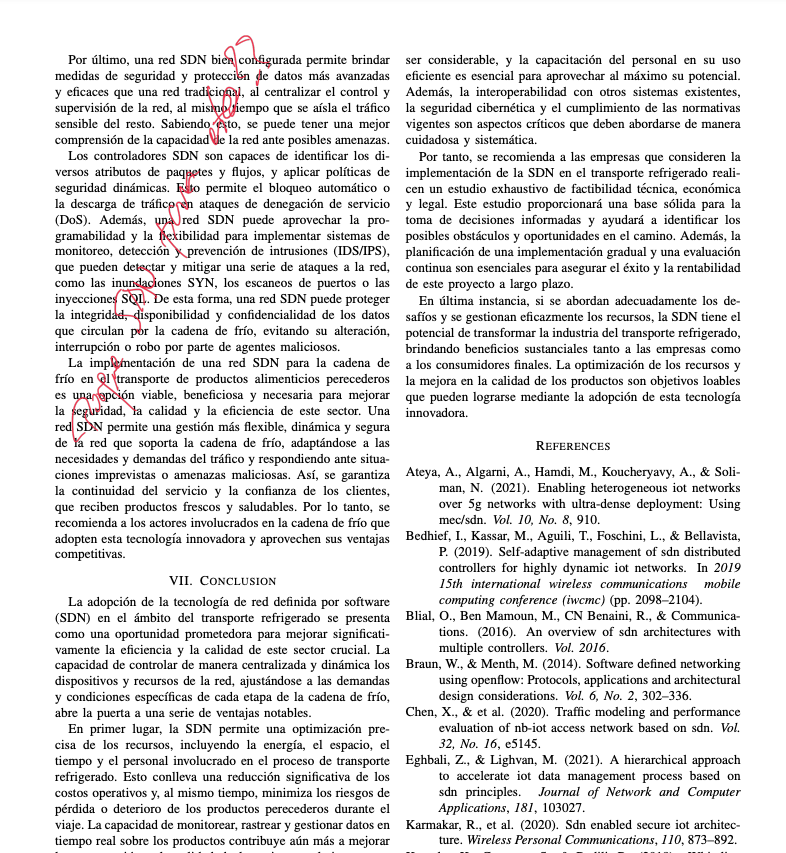
\includepdf[pages=-]{recursos/ra3/sto3a.pdf}


\newpage
\subsection{Resultado de aprendizaje \#: 7}
\label{sec:ra7}
T7: Discusión sobre Edge Computing

Actividad: Se debe realizar un discusión del tema del articulo propuesto, indicando los puntos más fuertes, las acciones, y las conclusiones del articulo. Asimismo, se debe buscar fuentes adicionales que permitan agregarle valor a la propuesta, e.g., Nuevos enfoques en el tema, nuevas técnicas que se podrían aplicar a la propuesta ó mejoras de la arquitectura propuesta basados en otras referencias científicas que sustenten los argumentos presentados en la discusión.

Antes de empezar la discusión, cada participante debe al menos interactuar "1 vez" para poder observar las respuestas de sus compañeros. 

Recurso: hu2019.pdf

Calificación:  Por pares (revisión cruzada) y por rúbrica. 

\subsubsection{Evidencia y retroalimentación RA7}
\begin{figure}[htbp]
    \centering
    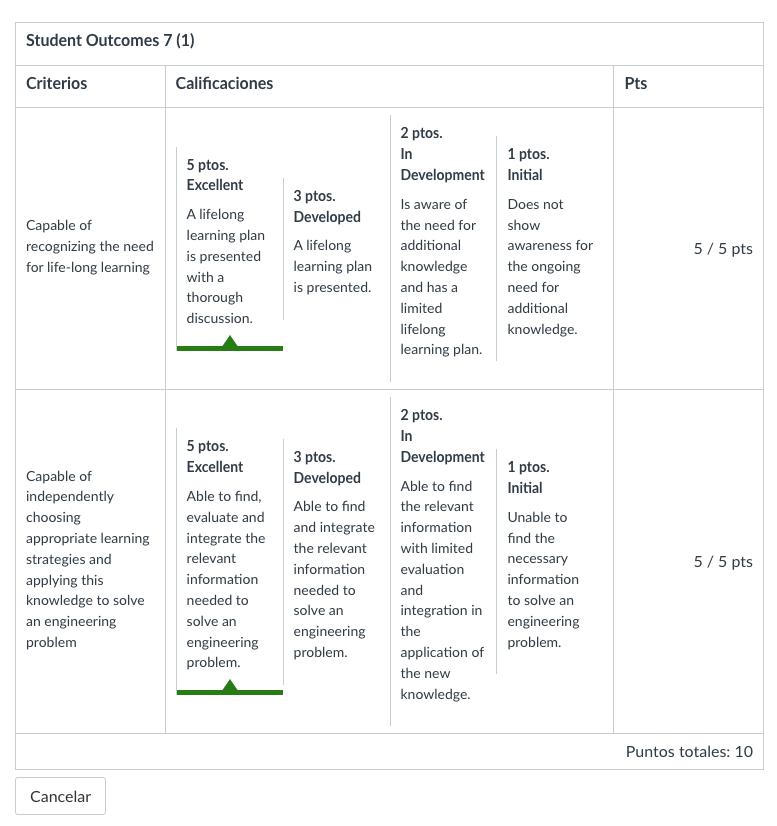
\includegraphics[width=\textwidth]{recursos/ra7/ra7-re.png}
\end{figure}

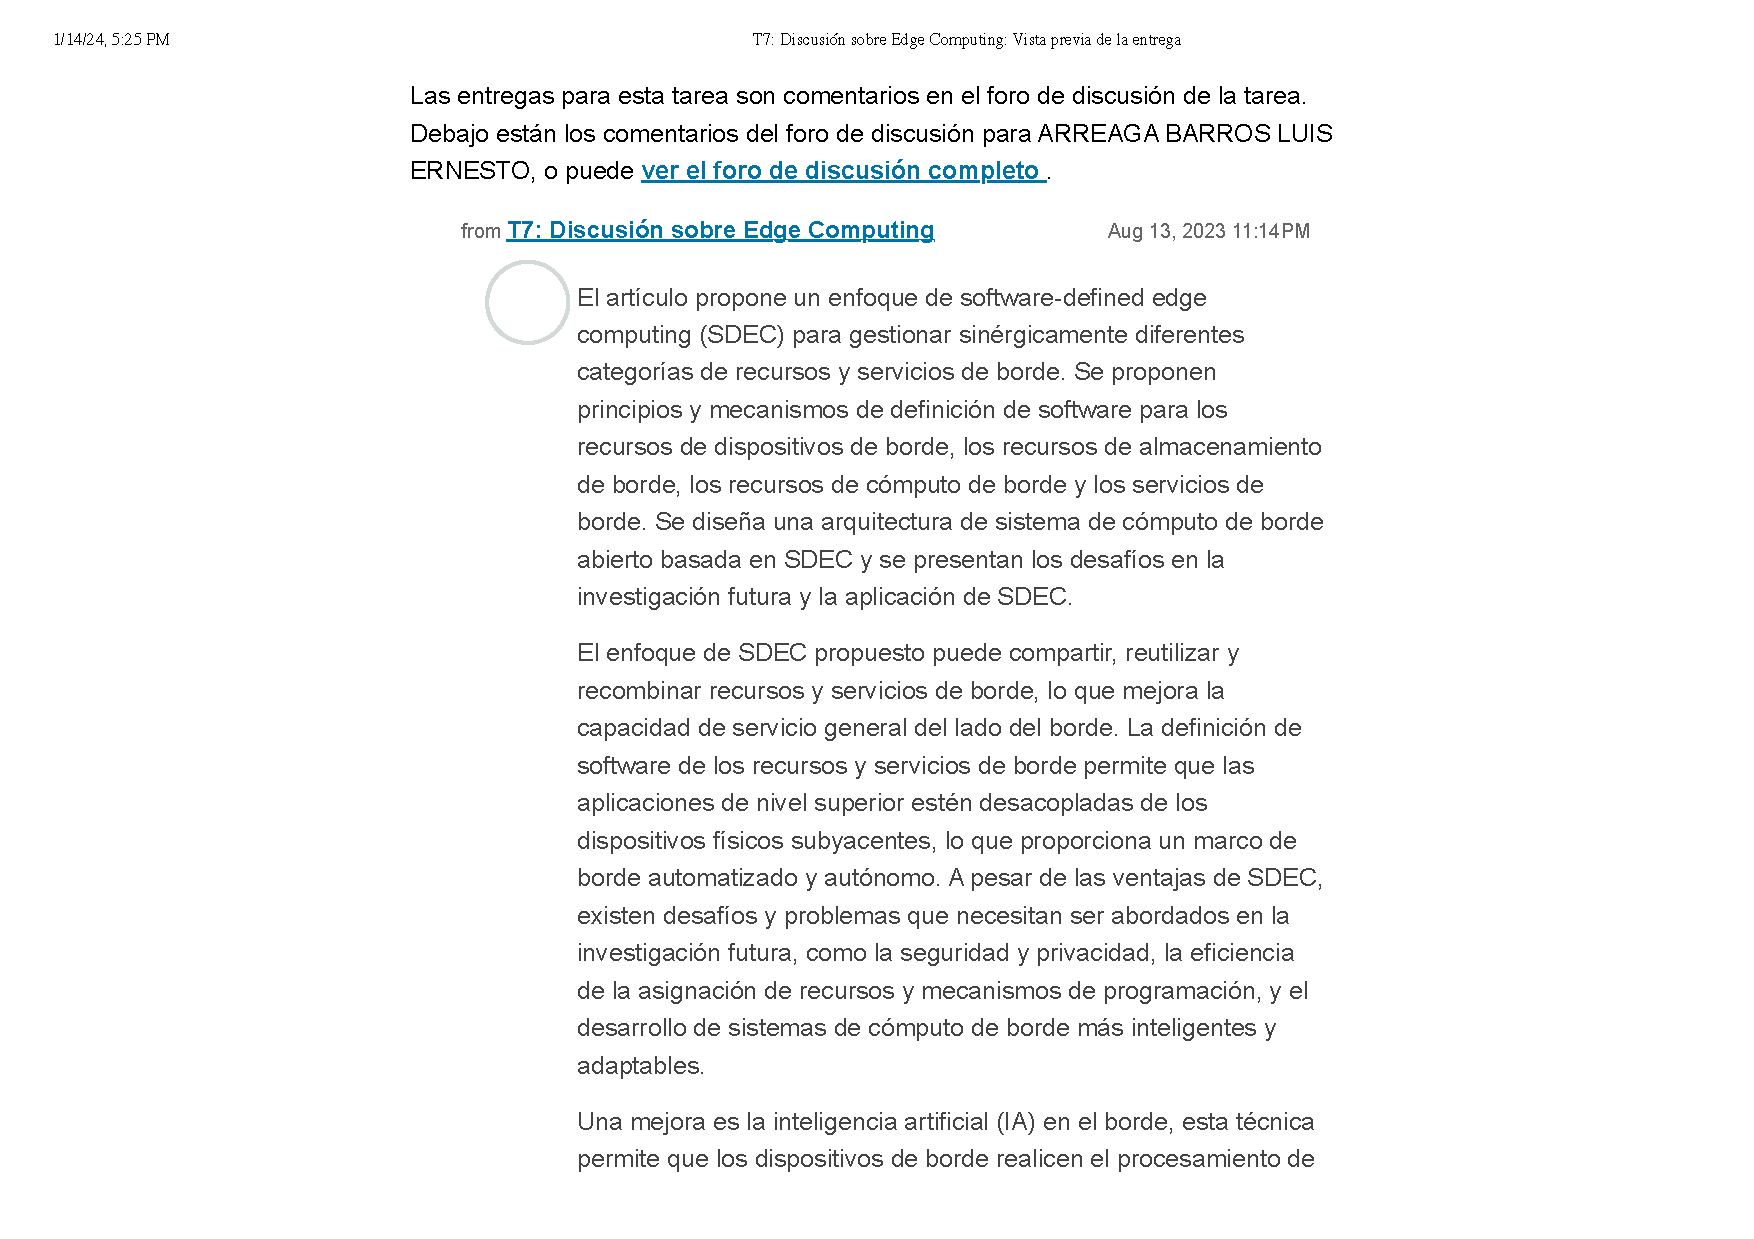
\includepdf[pages=-]{recursos/ra7/t7ev.pdf}